\documentclass[aps,prl,reprint,amsmath,amssymb]{revtex4-1}

\usepackage{epsfig,color,graphicx}
%\usepackage{algorithmic}
\usepackage{algorithm}
\usepackage{algpseudocode}

% Mathematical symbols
\newcommand*{\imi}{i} % imaginary i
\newcommand*{\E}{\mathrm{e}}
% DIRAC NOTATION
% bra-ket vectors
\newcommand{\ket}[1]{\ensuremath{\vert #1 \rangle}}
\newcommand{\bra}[1]{\ensuremath{\langle #1 \vert}}
\newcommand{\braket}[2]{\ensuremath{\langle #1 \vert #2 \rangle}} % bra-ket inner product
\newcommand{\ketbra}[2]{\ensuremath{\vert #1 \rangle \langle #2 \vert}} % ket-bra outer product
% operators
\newcommand{\op}[1]{\ensuremath{\hat{#1}}} % operator
\newcommand{\opsb}[2]{\ensuremath{\hat{#1}_{#2}}} % operator with subscript
\newcommand{\opsp}[2]{\ensuremath{\hat{#1}^{#2}}} % operator with superscript

% left-right arrow with text above it
\makeatletter
\newcommand\xleftrightarrow[2][]{%
  \ext@arrow 9999{\longleftrightarrowfill@}{#1}{#2}}
\newcommand\longleftrightarrowfill@{%
  \arrowfill@\leftarrow\relbar\rightarrow}
\makeatother

% inexact differential
\def\dbar{{\mathchar'26\mkern-12mu d}}

%partial derivative with some variables held constant
\newcommand{\pdc}[3]{\ensuremath{\left( \frac{\partial #1}{\partial #2} \right)_{#3}}}
\newcommand{\pddc}[3]{\ensuremath{\left( \frac{{\partial}^2 {#1}}{\partial {#2}^2} \right)_{#3}}}

%average
\newcommand{\av}[1]{\ensuremath{\left\langle{#1}\right\rangle}} % operator

%text color
\newcommand{\new}{\color{red}}
\newcommand{\blue}{\color{blue}}
\newcommand{\old}{\color{black}}

\begin{document}

\bibliographystyle{apsrev}


\title{
Direct unconstrained localization of one-electron orbitals
}

\author{Ziling Luo}
\email{ziling.luo@mail.mcgill.ca}
\author{Rustam Z. Khaliullin}
\email{rustam.khaliullin@mcgill.ca}
\affiliation{Department of Chemistry, McGill University, 801 Sherbrooke St. West, Montreal, QC H3A 0B8, Canada}

\date{\today}

\begin{abstract}
%RZZK: it is worth making the emphasis on the new approach to the localization procedure. Then say that, among other advantages, it is capable of producing more localized nonorthogonal orbitals.
Spatially localized one-electron orbitals are widely used in electronic structure theory to describe chemical bonding and speed up calculations.
Nonorthogonal localized molecular orbitals (NLMOs) are known to be noticeably more localized than their conventional orthogonal counterparts. 
Unfortunately, the existing methods to obtain NLMOs must pre-determine and freeze the localization center of each NLMO before its spread is minimized. 
This is done to avoid the ``collapse'' of the occupied subspace – a problem of NLMOs becoming linearly dependent. 
In this paper, we describe an unconstrained black-box method to localize nonorthogonal orbitals that determines the position of their centers automatically during the optimization process. 
The key to the new procedure is to construct and impose a penalty function which prevents the orbital ``collapse''. 
An algorithm is proposed to adjust the strength of the penalty and produce the right balance between orthogonality and locality of NLMOs. 
The resulting method produces NLMO fast, without requiring any \emph{a priori} knowledge of bonding patterns in the system (i.e. ``chemical intuition'') and is demonstrated to work well a variety of molecules and materials (RZZK: gamma-point only) including large systems with non-trivial bonding. 
\end{abstract}
%RZZK: mention nonorthogonal maximally localized Wannier functions in the abstract

\maketitle

\section{Introduction} 

% RZZK: Potential reviewers: Weitao?, Marzari, LMO for CP2K developers.

Spatially localized orbitals are of paramount importance in one-electron theories such as the Hartree-Fock (HF) method and Kohn-Sham density functional theory (DFT) as well as in post-HF wavefunction-based electron correlation methods.
Localized orbitals are widely used to describe and visualize chemical bonding between atoms thus helping classify bonds and understand electronic-structure origins of observed properties of atomistic systems. 
Furthermore, localized orbitals are the key ingredient in multiple local electronic structure methods~\cite{goedecker1994efficient, bowler2012methods, zalesny2011linear, pulay1986orbital, saebo2001low, pisani2005local, hampel1996local, forner1997numerical} that dramatically reduce the computational cost of modeling electronic properties of large atomistic systems.~\cite{saebo1993local, schutz1999low, hetzer2000low, schutz2001low}
Spatially localized orbitals are known as localized molecular orbitals (LMOs) in the field of molecular quantum chemistry and maximally localized Wannier functions (MLWFs) in solid state physics and materials science. 
Here, they will be collectively referred to as LMOs whereas the eigenstates of the effective one-electron Hamiltonian will be called canonical molecular orbitals (CMOs) regardless of whether the system is isolated or treated with periodic boundary conditions.

In traditional localization methods, LMOs are constructed by finding a unitary transformation of CMOs that minimizes a localization functional that effectively measures the spread of individual orbitals. 
Since CMOs are orthogonal and a unitary transformation preserves the overlap between orbitals, LMOs obtained in this way are orthogonal (OLMOs) by construction~\cite{weinstein1971localized}.
Multiple localization functionals have been proposed for molecular systems including Boys-Foster~\cite{boys1960construction}, Edmiston-Ruedenberg~\cite{bytautas2002electron, bytautas2003split, edmiston1963localized}, Pipek-Mezey~\cite{pipek1989a_fast}, and Von Niessen~\cite{niessen1972density}. The Boys-Foster localization~\cite{boys1960construction} is perhaps the most popular because of the simplicity of its physical interpretation, low computational complexity and ease of implementation. 
The Pipek-Mezey localization~\cite{pipek1989a_fast}, which maximizes atomic charges~\cite{mulliken1955electronic, lowdin1950non} of each orbital, is also widely used because it does not mix LMOs representing $\sigma$ and $\pi$ bonds and thus gives a clear picture of bonding patterns.
%guarantee that the $\sigma$-$\pi$ separation is always the stable solution compared with the mixed cases in OLMOs.
%
For condensed phase periodic systems, RZK.~\cite{marzari2012maximally}
%RZK: list and cite (reviews are preferred) appropriate localization methods (there should be one review by Nicola Marzari), mention Resta and Berghold.
% berghold2000general --- PHYSICAL REVIEW B, 61, 10040
% resta1999electron https://doi.org/10.1103/PhysRevLett.82.370
% resta1998quantum -- Phys. Rev. Lett. 80, 1800 (https://doi.org/10.1103/PhysRevLett.80.1800)
% silvestrelli1999maximally -- PRB 59 9703


While these methods rely on different localization criteria they all must ensure that orbitals remain orthogonal in the iterative localization procedure. This can be achieved through the exponential~\cite{RZK} or (RZK: other?) parameterization of unitary transformations or simple Jacobi rotations~\cite{RZK}.
%RZK: list most common methods that allow to maintain orthogonality. a good place to start is to read carefully the introduction of dx.doi.org/10.1021/ct400793q

Due to the imposed orthogonality condition, OLMOs exhibit small non-zero values even far away from the localization center. 
These orthogonalization tails can complicate the interpretation of chemically relevant electronic-structure information and make its transferability from one system to another more difficult. More importantly, the tails can reduce orbital locality making orbital-based local correlation methods less computationally efficient.
%
% To mitigate the undesirable orthogonality effects, it has been proposed to lift the orthogonality constraint during the localization procedure with the goal of increasing the flexibility and locality of LMOs. There are two distinct approaches to construct nonorthogonal LMOs (NLMOs). One approach bypasses CMOs and directly optimizes NLMOs that are constrained to a local space in the variational self-consistent filed (SCF) procedure~\cite{ZZZ}. Unfortunately, the localization constraints imposed on NLMOs can result in the NLMO energy being substantially higher than that of the fully delocalized state. Another approach is to obtain NLMOs is a post-SCF localization procedure that finds a nonsingular transformation of CMOs. 
% 
To mitigate the undesirable orthogonality effects, it has been proposed to replace a unitary transformation of CMOs with a more general nonsingular transformation. This generalization lifts the orthogonality constraint in the localization procedure and increases the number of degrees of freedom available to LMOs~\cite{anderson1968self, diner1968fully, magnasco1974localized, payne1977hartree, mehler1977self, feng2004An_efficient, cui2010efficient}. 
It has been found that NLMOs are indeed about $10-30 \%$ more localized than OLMOs if measured by the value of the Boys-Foster functional~\cite{feng2004An_efficient, liu2000nonorthogonal}. %(RZK: check whether the Boys-Foster functional is used indeed)  

Substantial recent efforts have been made to develop reliable algorithms to construct NLMOs~\cite{feng2004An_efficient, liu2000nonorthogonal, peng2013effective, hoyvik2017generalising}. 
%
Despite noticeable progress the existing methods produce NLMOs that are either still fairly similar to OLMOs 
[RZK: do we have a citation for this?] 
or lead to the linear dependence between the orbitals~\cite{feng2004An_efficient}. 
To overcome the widespread linear dependence problem, Yang and co-workers~\cite{feng2004An_efficient, cui2010efficient} have developed a localization method in which the centers of NLMOs are fixed during the minimization of the localization functional. 
The positions of the centers are predefined using those of the corresponding OLMOs~\cite{feng2004An_efficient} or simply guessed based on the knowledge of bonding patterns in a system~\cite{cui2010efficient}. %(i.e.``chemical intuition'')
While this method solves severe linear dependence issues, it requires either computational efforts to construct OLMOs centroids or good understanding of bonding properties in advance,which may limit the application of the method to relatively simple systems.

In this paper, we propose a new approach to simplify the construction of LMOs. 
The key new component of the method is a penalty function that prevents LMOs from becoming linear dependent.  
An algorithm for adjusting the penalty strength allows to choose the desirable balance between the nonorthogonality and locality of LMOs. 
For OLMOs, the method is advantageous because it optimizes orbital mixing coefficients directly, obviating complicated parameterization of unitary transformations and simplifying optimization algorithms significantly.  
For NLMOs, the new approach allows to determine the optimal positions of their centers automatically in an unconstrained and straightforward optimization procedure, without \emph{a priori} knowledge of bonding patterns in the system.
The proposed localization method is demonstrated to work well for a variety of molecules and materials including large systems with non-trivial bonding. 


\section{Theory and algorithms}

The localization procedure starts with a set of occupied one-electron states $\ket{i_0}$. 
These orbitals are not assumed to be canonical or even orthogonal. 
However, they are assumed to be normalized, which does not reduce the generality of the method. 
Furthermore, the initial orbitals must be linear independent, that is, their overlap matrix $\sigma_{ji}^0 \equiv \braket{j_0}{i_0}$ must be invertible. 
The trial NLMOs are expressed as a linear combination of these initial states
%
\begin{equation}
\begin{split}
\ket{j} = \ket{i_0} {A^i}_j  
\end{split}
\end{equation}
%
The conventional tensor notation is used to work with the nonorthogonal orbitals~\cite{head1998tensor}: covariant quantities are denoted with subscripts, contravariant quantities with superscripts, and summation is implied over the same orbital indices.

The objective function minimized in this work contains two terms: a conventional localization functional $\Omega_L$ and a term that penalizes unphysical states with linearly dependent occupied orbitals $\Omega_P$:
%
\begin{equation} \label{eq:fun-pen}
\begin{split}
\Omega(\mathbf{A}) = \Omega_L(\mathbf{A}) + c_P \Omega_P(\mathbf{A}), \\
\Omega_P(\mathbf{A}) = - \log \det \left[ \sigma (\mathbf{A}) \right]
\end{split}
\end{equation}
%
where $c_P > 0$ is the penalty strength, $\sigma$ is the NLMO overlap matrix 
%
\begin{equation}
\begin{split}
\sigma_{kl} = \braket{k}{l} = {A^j}_k \sigma_{ji}^0{A^i}_l
%= (\mathbf{A}^\dagger \mathbf{T}^\dagger \mathbf{ S T A})_{kl},
\end{split}
\end{equation}
%

If the NLMOs are normalized the determinant of $\sigma$ varies from 1 for orthogonal NLMOs to 0 for linearly dependent NLMOs. The penalty function---the key ingredient of the proposed method---varies from 0 to $+\infty$ for these two extreme cases, making linearly dependent state inaccessible in the localization procedure with finite penalty strength $c_P$. 
% RZZK: Why sigma instead of A? quadratic penalty in terms of A (more complicated in terms of a). Why log?
A normalization constraint can be imposed on NLMOs if their coefficients are expressed in terms of independent variational parameters denoted with lowercase $\mathbf{a}$
%
\begin{equation}
\begin{split}
{A^i}_j = {a^i}_{j} ({a^k}_{j} \sigma^0_{kl}{a^l}_{j})^{-\frac{1}{2}} \equiv {a^i}_{j} N_j ,
\end{split}
\end{equation}
%
where the $\mathbf{a}$-dependent normalization coefficient $N_j$ is defined for brevity. 

The inclusion of the penalty term converts the localization procedure into an unconstrained and straightforward optimization problem. Additionally, adjusting the strength of the penalty $c_P$ enables one to achieve the right balance between the nonorthogonality and locality of the orbitals (see below). 

In this work, we adopted the localization functional proposed by Resta~\cite{resta1998quantum, resta1999electron} and generalized by Berghold \emph{et al.}~\cite{berghold2000general} to three dimensions and simulation cells of general shape and symmetry: 
%
% RZK: do we really use log function? If not, fix the gradient (PM and Boys are consistent then) and re-write the PM section to include only the kernel instead of all three equation (alpha->K). If yes, the PM gradient must be different.
\begin{equation} \label{eq:fun-loc}
\begin{split}
\Omega_L(\mathbf{A}) &= - \sum_K \sum_i \omega_K \log \vert z_{i}^{K} \vert^2, \\
z_{i}^{K} &= {A^m}_i B^{K}_{mn} {A^n}_i, \\
B^{K}_{mn} &= \bra{m_0} \E^{\imi \mathbf{G}_K \cdot \mathbf{\op{r}}} \ket{n_0}
\end{split}
\end{equation}
%
where $\mathbf{\op{r}}$ is the position operator in three dimensions, $\omega_K$ and $\mathbf{G}_K$ are suitable sets of weights and reciprocal lattice vectors, respectively, labeled by index $K$~\cite{silvestrelli1999maximally, berghold2000general}. We chose to write the summation over $K$ explicitly because $K$ is not an orbital index. The functional in Eq.~(\ref{eq:fun-loc}) can be used for both gas-phase and periodic systems~\cite{berghold2000general}. In the former case, the functional is equivalent to the Boys-Foster localization~\cite{berghold2000general, resta1999electron}. In the latter case, its applicability is limited to the electronic states described within the $\Gamma$-point approximation.

We also considered the Pipek-Mezey localization functional~\cite{pipek1989fast,lehtola2014pipek} that has the advantage of preserving the separation of $\sigma$ and $\pi$ bonds and is commonly employed for molecular system
%
\begin{equation} \label{eq:pipek}
\begin{split}
\Omega_L^{\text{PM}}(\mathbf{A}) &= - \sum_{\alpha=1}^{\text{Atoms}} \sum_i \vert z_{i}^{\alpha} \vert^2, \\
z_{i}^{\alpha} &= {A^m}_i B^{\alpha}_{mn} {A^n}_i, \\
B^{\alpha}_{mn} &= \frac{1}{2} \sum_{\mu \in \alpha} \bra{m_0}  \left( \ketbra{\chi_{\mu}}{\chi^{\mu}} + \ketbra{\chi^{\mu}}{\chi_{\mu}} \right) \ket{n_0}
%RZZK alpha and mu do not belong to the same set
\end{split}
\end{equation}
%
%
where $z_{i}^{\alpha}$ is the contribution of orbital $i$ to the Mulliken charge of atom $\alpha$, $\ket{\chi_\mu}$ and $\ket{\chi^\mu}$ are atom-centered covariant and contravariant basis set functions~\cite{silvestrelli1999maximally, berghold2000general}. The summation over $\mu$ is written explicitly to emphasize that it is restricted to the basis functions centered on atom $\alpha$. 

%RZZK: PM discussion

The unconstrained minimization of functional $\Omega$ with fixed $c_P$ can be carried out with a variety of algorithms. In this work, we used a simple conjugate gradient algorithm summarized in Figure~\ref{fig:cg}. The gradient ${G_i}^j \equiv \frac{\partial \Omega}{\partial {a^i}_j}$  required in the algorithm is a sum of the localization ${L_i}^j \equiv \frac{\partial \Omega_L}{\partial {a^i}_j}$ and penalty ${P_i}^j \equiv \frac{\partial \Omega_P}{\partial {a^i}_j}$ components
%
\begin{equation} \label{eq:grad}
\begin{split}
G{_k}^{l} = L{_k}^{l} + c_P P{_k}^{l}.
\end{split}
\end{equation}
%
These components can be readily expressed in terms of the derivatives with respect to the transformation coefficients $\tilde{X}{_k}^l \equiv \frac{\partial \Omega_X}{\partial {A^k}_l}$, where $X$ is either $L$ or $P$:
%
\begin{equation} \label{eq:grad-convert}
\begin{split}
{X_i}^j & = \tilde{X}{_k}^l \frac{\partial {A^k}_l}{\partial {a^i}_j} = \left[ \tilde{X}{_i}^j - ( \sigma_{in}^0 {A^n}_j ) ( {A^m}_j \tilde{X}{_m}^j ) \right] N_j 
\end{split}
\end{equation}
%
\begin{equation} \label{eq:grad-loc}
\begin{split}
\tilde{L}{_k}^l & = - \sum_K \frac{4 \omega_K}{\vert z_{l}^{K} \vert^2} \times \\ 
&\times \left[  \operatorname{Re}(B^{K}_{kn}) {A^{n}}_{l} \operatorname{Re}(z_{l}^{K}) + \operatorname{Im}(B^{K}_{kn}) {A^{n}}_{l} \operatorname{Im}(z_{l}^{K}) \right]
\end{split}
\end{equation}
%
\begin{equation} \label{eq:grad-pen}
\begin{split}
\tilde{P}{_k}^l & = -2 \sigma_{km}^0 {A^m}_n \sigma^{nl} 
\end{split}
\end{equation}
%

\textbf{Penalty strength.} If the penalty strength $c_P$ is extremely large, $\Omega_L$ is negligible compared to the penalty term and the minimization of $\Omega$ is numerically equivalent to a trivial orbital orthogonalization. In the opposite case of extremely small $c_P$, the minimization of $\Omega$ may result in a linear dependence between NLMOs as reported earlier~\cite{cui2010efficient}. 
In the latter case, the algorithm shown in Figure~\ref{fig:cg} fails to compute the inverse of the NLMO overlap required in Eq.~(\ref{eq:grad-pen}) and stops. 

As we show below, there is a wide range of $c_P$ values between the two extremes that produce NLMOs that are substantially more localized than OLMOs and linearly independent.  
%
A simple strategy to find an appropriate penalty strength is to minimize $\Omega$ with a sufficiently large initial $c_P$ value and then gradually decrease $c_P$ until the determinant of the overlap of the \emph{optimal} NLMOs drops below a desired threshold $\text{D}_{\text{min}} \in (0,1]$. 
The initial value of $c_P$ should be chosen to balance approximately the localization and penalty components of $\Omega$. 
Thus, a reasonable initial value of $c_P$ can be estimated by assuming that the reduction in $\Omega_L$ upon the minimization of $\Omega$ has the same order of magnitude as the change in the penalty $c_P \Omega_P$:
%
\begin{equation} \label{eq:cp-beta}
\begin{split} 
%\Omega_L(\mathbf{I}) + c_P \Omega_P(\mathbf{I}) & \sim \Omega_{L}(\mathbf{A}^{\ast}) - c_P \log \text{D}_{\text{min}} \\
c_P^{\text{init}} & \sim \frac{ \Omega_{L}(\mathbf{I}) - \Omega_{L}(\mathbf{A}^{\ast}) }{ \Omega_{P}(\mathbf{A}^{\ast}) - \Omega_{P}(\mathbf{I}) } = \frac{ \beta_L^{\ast} }{ \beta_P^{\ast} } \times \Omega_{L}(\mathbf{I})
\end{split}
\end{equation}
%
where $\mathbf{A}^{\ast}$ denotes the (yet unknown) solution to the minimization problem, 
%
\begin{equation} 
\begin{split} 
\beta_L^{\ast} \equiv \frac{\Omega_L(\mathbf{I})- \Omega_L(\mathbf{A}^{\ast})}{\Omega_L(\mathbf{I})} \in [0,1]
\end{split}
\end{equation}
%
is the (positive) expected relative reduction in the localization functional, and 
%
\begin{equation} \label{eq:betap}
\begin{split} 
\beta_P^{\ast} \equiv \log \frac{\det \sigma(\mathbf{I})}{ \det \sigma(\mathbf{A}^{\ast}) } \approx \log \frac{\det \sigma(\mathbf{I})}{ \text{D}_{\text{min}} } \equiv \beta_P > 0
\end{split}
\end{equation}
%
is the logarithm of the ratio of the initial and final determinants. 
The importance of Eqs.~(\ref{eq:cp-beta})--(\ref{eq:betap}) is that they allow to estimate the initial value of $c_P$ as a product of $\Omega_L(\mathbf{I})$, which can be easily calculated in the beginning of the optimization procedure, and a dimensionless constant $\alpha$
%
\begin{equation} \label{eq:cp-alpha}
\begin{split}
c_{P}^{\text{init}} = \frac{ \beta_L^{\ast} }{ \beta_P } \times \Omega_L(\mathbf{I}) \equiv \alpha \times \Omega_L(\mathbf{I})
\end{split}
\end{equation}
%
Eq.~(\ref{eq:cp-alpha}) makes clear that the penalty component is an extensive function of a system with the units that are consistent with the localization component. Although the optimal dimensionless parameter $\beta_L^{\ast}$ is not known \emph{a priori} its magnitude can be easily estimated to obtain a sufficiently large initial guess for $c_P$. For example, an optimization of canonical orbitals $\det \sigma(\mathbf{I})=1$ that stops when the NLMO determinant drops below $\text{D}_{\text{min}} = 0.1$ can be initialized by adopting the maximum possible value of $\beta_L^{\ast} = 1$ that results in $\alpha = \log^{-1} 10$.

The procedure for tuning $c_P$ is shown as the outer loop of the algorithm in Figure~\ref{fig:cg}. Its only required input is $\text{D}_{\text{min}}$. % Parameter $\alph$ is then computed using Eq.~(\ref{eq:cp-alpha}). Alternatively, parameter $\alpha$ can be specified as an input. It is also %RZZK

%RZZK: Depending on the results discuss the following: If the precise value of the determinant is necessary the penalty can be replaced with c_P becoming a Langrange multiplier that can be determined precisely. In a MD or geopt, determine $c_P$ once and then fix it for subsequent geometries. This is valid as long as the electronic properties of the system remain the same (e.g. there is not insulator to metal phase transition). 

%RZZK: Dmin is a misnomer.

\begin{figure}
\begin{algorithm}[H]
  \caption{Conjugate gradient minimization of $\Omega$}
  \label{alg:cg}
   \begin{algorithmic}[1]
   	%\Procedure{Minimize$\Omega$}{$c_P, \tau, \mathbf{T}_0$}
	\State Input $\epsilon_{\text{CG}}$ \Comment{Localization convergence threshold}
	%\State Input $N_{\text{CG}}$, $N_{\text{Outer}}$ \Comment{Max CG, outer iterations}
	\State Input $\text{D}_{\text{min}}$ \Comment{Minimum allowed NLMO determinant}
   	\State Input $\mathbf{T}_0$ \Comment{Initial basis set coefficients for $\ket{i_0}$}
   	\State Input $\mathbf{S}$ \Comment{Basis set overlap}
   	\State Input $\mathbf{L}^K$ \Comment{Basis set representation of the localization operator} 
   	\State $\mathbf{\sigma}_0 \gets \mathbf{T}_0^{\dagger} \mathbf{ST}_0$ \Comment{Initial orbital overlap} 
   	\State $\mathbf{B}^{K} \gets \mathbf{T}_0^{\dagger} \mathbf{L}^K \mathbf{T}_0$ \Comment{Initial localization matrix, Eq.~(\ref{eq:fun-loc})} 
	\State $\mathbf{a} \gets \mathbf{I}$ \Comment{Initial guess on variational parameters}
	%\State Converged $\gets$ False
	\State StopOuter $\gets$ False \Comment{Flag to exit the outer loop}
	\State $i_{\text{Outer}} \gets 0$ \Comment{Iteration counter}
	\Repeat \Comment{Loop to change the penalty strength}
		\State $i_{\text{Outer}} \gets i_{\text{Outer}} + 1$ 
		\State StopCG $\gets$ False \Comment{Flag to exit the CG loop}
		\State $i_{\text{CG}} \gets 0$ \Comment{Iteration counter}
%		\State $\beta \gets 0$ \Comment{Reset conjugation}
		\Repeat \Comment{Fixed-penalty localization loop}
			\State $i_{\text{CG}} \gets i_{\text{CG}} + 1$ 
			\State $\mathbf{A} \gets \mathbf{a} \left[ \text{diagonal}(\mathbf{a}^{\dagger} \mathbf{\sigma}_0 \mathbf{a}) \right]^{-\frac{1}{2}}$ \Comment{Update NLMOs}
			\State $\mathbf{\sigma} \gets \mathbf{A}^{\dagger}\mathbf{\sigma}_0 \mathbf{A}$ \Comment{Update overlap}
			\State $\text{Det} \gets \text{determinant} (\mathbf{\sigma})$ \Comment{Determinant}
			\State $\Omega_{P} \gets - \log [\text{Det}] $ \Comment{Orthogonalization functional}
			\State $\mathbf{P} \gets \text{Eq~(\ref{eq:grad-pen}) and~(\ref{eq:grad-convert})}$ \Comment{Orthogonalization gradient}
			\State $\Omega_{L} \gets \text{Eq~(\ref{eq:fun-loc})}$ \Comment{Localization functional}
			\State $\mathbf{L} \gets \text{Eq~(\ref{eq:grad-loc}) and~(\ref{eq:grad-convert})}$ \Comment{Localization gradient}
			\If{$i_{\text{Outer}}=1$ \textbf{and} $i_{\text{CG}}=1$} 
				%\State $c_{P} \gets \text{Tr}(\mathbf{L}^{\dagger} \mathbf{P})/\text{Tr}(\mathbf{P}^{\dagger}\mathbf{P})$
				\State $c_{P} \gets \Omega_{L}(\log [\text{Det} / \text{D}_{\text{min}} ])^{-1}$ \Comment{Initial strength}
			\EndIf
			\State $\Omega \gets \Omega_{L} + c_P \Omega_{P} $ 
			\If{$i_{\text{CG}}>1$}
				\State $\mathbf{\Gamma} \gets \mathbf{G}$ \Comment{Save old gradient}
			\EndIf 
			\State $\mathbf{G} \gets \mathbf{L} + c_P \mathbf{P} $ 
			%\State $\text{Error}_\text{CG} \gets \vert\vert \mathbf{G} \vert \vert_{\text{max}}$
			\If{$\vert\vert \mathbf{G} \vert \vert_{\text{max}} < \epsilon_{\text{CG}}$}
				\State StopCG $\gets$ True
			\EndIf
%			\If{$i_{\text{CG}}=1$ \textbf{And} $i_{\text{Outer}}=1$}
%				\State StopCG $\gets$ False \Comment{Do first iteration}
%			\EndIf
			\If{\textbf{not} StopCG}
%				\If{$i_{\text{CG}} = 1$}
%					\State $\mathbf{P}^{R_c} \gets \text{Eq.\ref{eq:prec}}(\mathbf{F},\mathbf{M}^{R_c},\mathbf{K}^{R_c}) $\Comment{Precon.}
%				\Else
%					\State $\mathbf{O}_{R_c} \gets \mathbf{D}_{R_c}$ \Comment{Save old direction}
%				\EndIf
				\If{$i_{\text{CG}} > 1$}
					\State $\mathbf{O} \gets \mathbf{D}$ \Comment{Save old direction}
				\EndIf
%				\State $\mathbf{D}_{R_c} \gets - [(\mathbf{P}^{R_c})^{-1} \mathbf{G}^{R_c}]_{R_c}$ \Comment{Precon. grad.}
				\State $\mathbf{D} \gets - \mathbf{G}$ \Comment{Initial direction}
				\If{$i_{\text{CG}}>1$}
					\State $\beta \gets \text{Tr}(\mathbf{G}^{\dagger} \mathbf{D})/\text{Tr}(\mathbf{\Gamma}^{\dagger}\mathbf{O})$
					\State $\mathbf{D} \gets \mathbf{D} + \beta \mathbf{O}$ \Comment{Search direction}
				\EndIf 
				\State $\alpha \gets \text{argmin}_{\alpha} \Omega(\mathbf{a} + \alpha \mathbf{D})$ \Comment{Line search}
				\State $\mathbf{a}\gets \mathbf{a} + \alpha \mathbf{D}$ \Comment{Update variational DOFs}
			\EndIf
		\Until{StopCG} 
%RZZK: add an additional criterion that prevents high-determinant cases go on forever
		%\If{$\text{Det} < \text{Det}_{\text{Target}}$ \textbf{or} $i_{\text{Outer}} > N_{\text{Outer}}$}
		\If{$\text{Det} < \text{D}_{\text{min}}$}
			\State StopOuter $\gets$ True
		\EndIf
		\If{$i_{\text{Outer}}>1$} 
			\State $c_{P} \gets c_P / RZK$ \Comment{Reduce $c_P$}
		\EndIf
	\Until{StopOuter}
	\State $\mathbf{return}$ $\mathbf{T} \gets \mathbf{T}_0 \mathbf{A} $ \Comment{Return NLMOs coefficients}
	%\EndProcedure
   \end{algorithmic}
\end{algorithm}
\caption{\label{fig:cg} Algorithm for the optimization of NLMOs.}
\end{figure}

\textbf{Implementation.} The localization procedure was implemented in the CP2K software package~\cite{cp2kgeneral}. The DBCSR library~\cite{borstnik2014sparse} that handles sparse matrices efficiently on massively-parallel computing platforms is utilized to enable orbital localization in large systems.
%borstnik2014sparse - https://doi.org/10.1016/j.parco.2014.03.012

%RZZK: Describe our recursive procedure for quick and reliable linear-scaling determinant evaluation.


\section{Results and discussion}

\subsection{Computational details}

To test the localization procedure, we constructed NLMOs for several systems ranging from a simple water molecule to complex molecules with non-trivial bonding patterns and to large periodic systems. 
%
For all systems, the initial CMOs were obtained using the conventional diagonalization-based SCF procedure implemented in the DFT module of CP2K. 
The Becke-Lee-Yang-Parr generalized gradient approximation~\cite{becke1988density, lee1988development} was used as the exchange-correlation functional.
Goedecker-Teter-Hutter pseudopotentials~\cite{goedecker1996separable} were used together with a triple-$\zeta$ atom-centered Gaussian basis set with two sets of polarization functions for all atoms. 
The energy cutoff was set at 600 Ry to define the auxiliary plane-wave basis set in the construction of the effective Hamiltonian. 
The integration over the Brillouin zone was performed using the $\Gamma$-point approximation.

% RZK: The plan is:
%*** Demonstrate how the penalty-strength algorithm works with the default and user-specified input parameters: $\alpha$, D$_{\text{min}}$, reduction factor. For selected, illustrative examples present figures showing optimal NLMO localization and determinant as a function of $c_P$.
%*** Compare the spread (what do we use as the spread proxy?) of CMOs, OLMOs, NLMOs for simple systems. The main question is whether relaxation of the centroid position allows to achieve better localization. Perhaps not. 
%*** Demonstrate that the new scheme reproduces the expected localization on bonds. Show graphene example.
%*** Show how the new scheme works for more complex systems. Borans and carboranes.
%*** Illustrate reduction in the orthogonalization tails.
%*** Anything else?

\subsection{Compromise between locality and orthogonality}

For all test systems, the conjugate gradient localization procedure in Figure~\ref{alg:cg} is stable and efficient. The numerical precision of the implemented code allows to treat NLMOs with $\det(\sigma)$ as lows as $10^{-8}$ as linearly independent. However, a visual inspection of NLMOs with such a tiny overlap determinant reveals that orbitals can become almost identical (for example, localized on the same bonds) with only minor physically irrelevant differences. At the same time, NLMOs with $\det(\sigma) > 10^{-1}$ are found to highlight bonding patterns in all test systems correctly. Therefore, we set the minimum allowed NLMO determinant $\text{D}_{\text{min}}$ to $10^{-1}$ in all tests. The initial value of $\alpha=\log^{-1} 10$ was set according to Eq.~(\ref{eq:cp-alpha}). The value of $\alpha$ was decreased by a factor of RZK in the outer loop of the algorithm (Figure~\ref{alg:cg}) until the overlap determinant fell below $\text{D}_{\text{min}}$ or until the optimal $\Omega_{L}$ stopped changing with $c_P$ appreciably (see water, diborane, heptane examples in Figure~\ref{fig:alpha}). 

%RZZK: details on the second "stop early" criterion for c_P adjustment

It is important to note that the determinant of the overlap is proportional to the square of the volume of the multidimensional parallelepiped spanned by the NLMO vectors defined by matrix $\mathbf{A}$. If the initial orbitals are orthonormal with $\det(\sigma^0)=1$, which is the case here, $\text{D}_{\text{min}}=10^{-1}$ corresponds to the parallelepiped volume of $\det(\mathbf{A})\approx 0.32$ that is large enough to produce distinct NLMOs.

\begin{figure*}[hbpt]
\centering
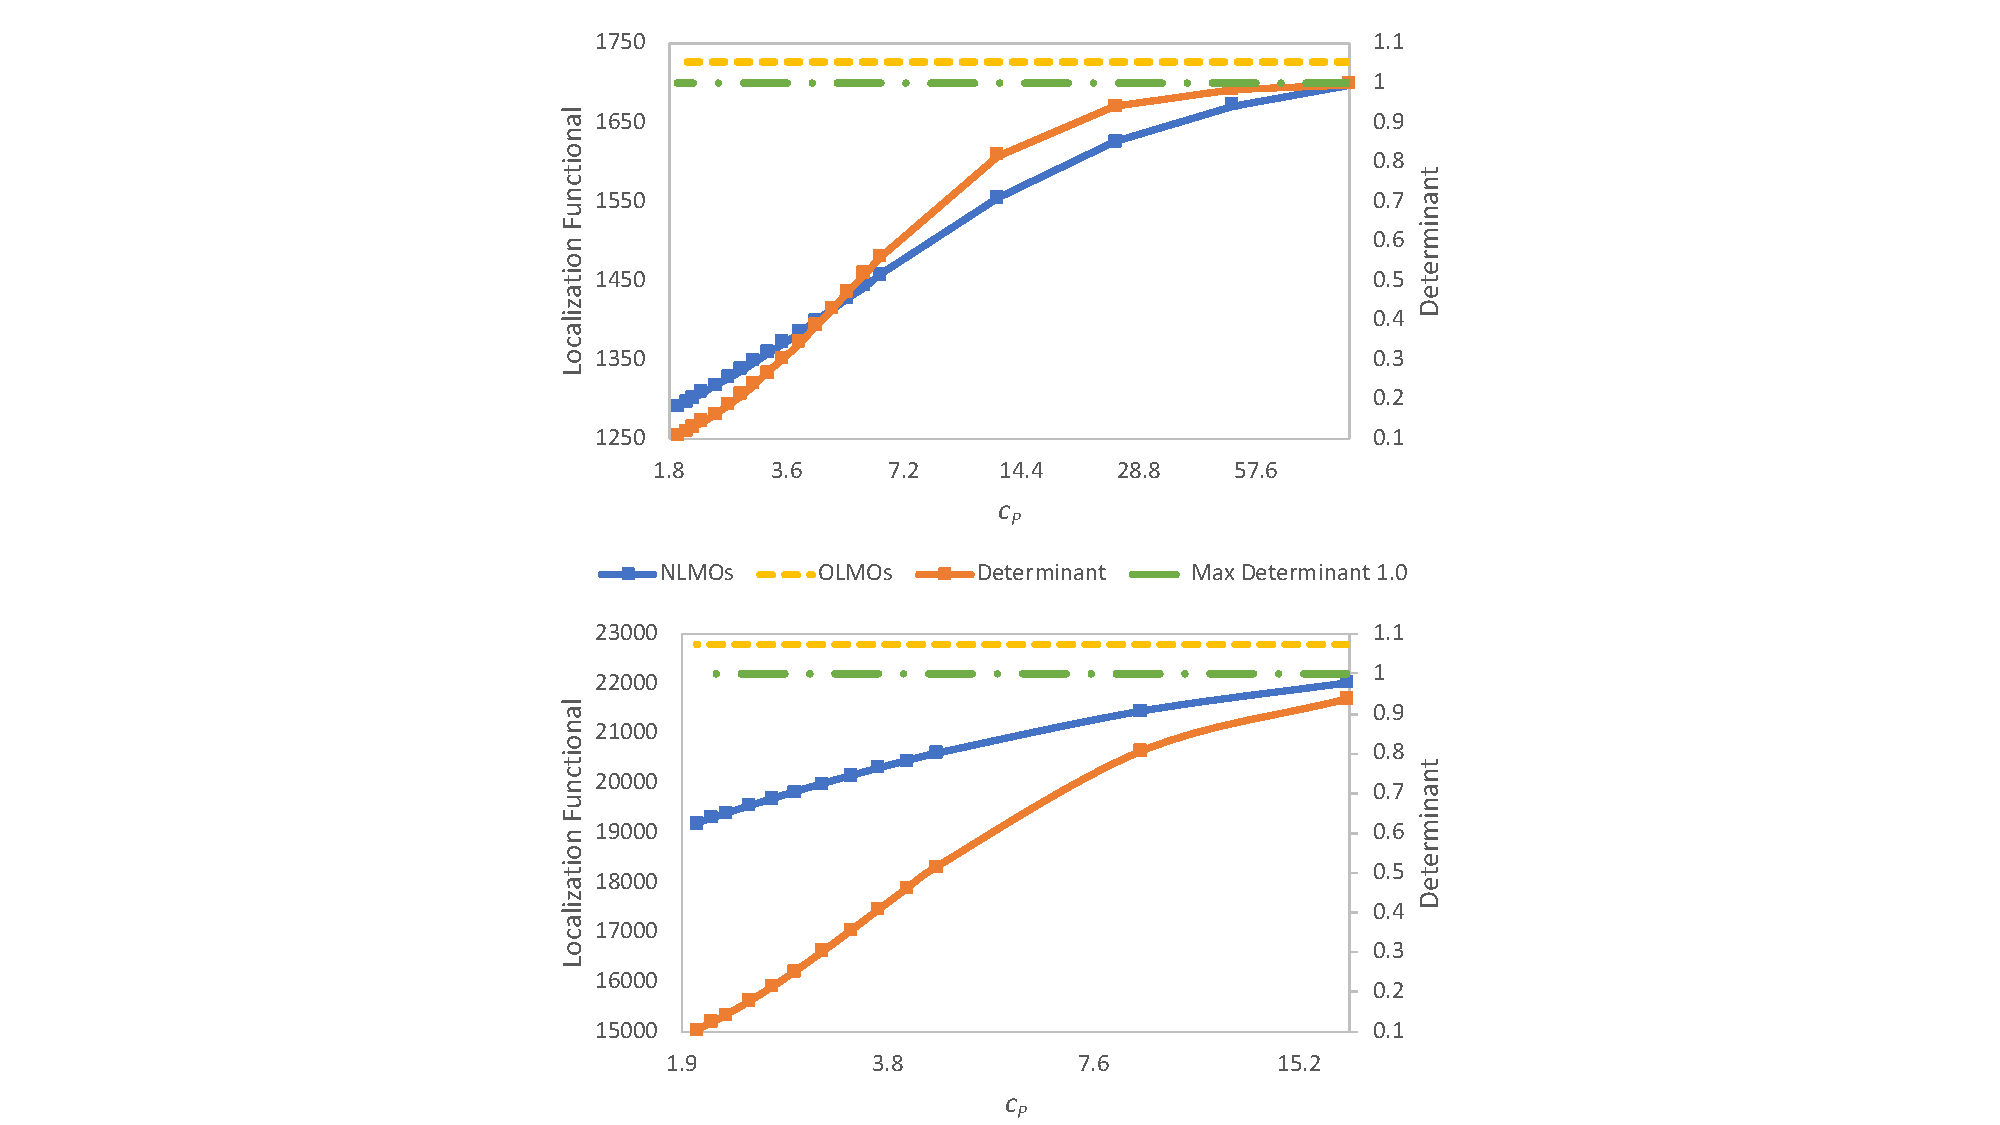
\includegraphics[width=\textwidth]{figure_2.pdf}
\caption{The dependence of the optimal localization functional and determinant of the NLMO overlap on $\alpha$ -- the adjustable part of the penalty strength. The first point on the left is $\alpha = \log^{-1} 10 \approx 0.434$. 
RZK: Icosane does not start at this alpha. We need to formulate a clear stopping criterion in cases where the alpha decrease does not lower the determinant to Dmin (water, diborane, heptane). Perhaps we can demonstrate that we can stop early by truncating the flat regions at small alpha. Use different symbol shape for one of the lines.}
\label{fig:alpha}
\end{figure*}

Figure~\ref{fig:alpha} demonstrates how the penalty strength affects the optimal orbital localization and the determinant of the orbital overlap. In all tests, the initial penalty strength is sufficiently large to produce almost perfectly orthogonal localized orbitals. At the same time it is not too large to yield more localized linearly independent nonorthogonal localized orbitals after just several steps of $c_P$ adjustment. %Figure~\ref{fig:alpha} shows that $c_P$ can be adjusted with a black-box algorithms to generate linearly independent NLMOs.

Figure~\ref{fig:alpha} shows that within a large range of values spanning 3--6 orders of magnitude $c_P$ serves as an adjustable parameter that can be tuned to achieve a desirable locality-orthogonality compromise. 
Thus the flexibility of the unconstrained localization method presented here allows to combine the strengths of the existing localization methods that produce either orthogonal orbitals or NLMOs with fixed localization centers. It is also important to emphasize that the localization procedure is unconstrained, does not require complicated parameterization of unitary matrices and relies on a simple easy-to-implement conjugate gradient optimization algorithm. 

%RZZK-toTheory? Furthermore, the presented approach can be modified to treat $c_P$ as a Lagrange multiplier that restraints the overlap determinant to a desirable value.

\subsection{NLMOs are more localized than OLMOs}

% RZZK: use beta values defined in the equations above instead of percentage redaction, a priori and posteriori values of alpha

\begin{table*}[htbp]
\caption{The relative reduction in the localization functional and the final determinant of the NLMO overlap. RZK: reduce Deltas to two significant digits and switch to percentage scale (see water and CO2 as an example).}
\label{tab:loc}
\centering
\begin{tabular}{l c c c c}
\hline\hline
Molecules & $\Delta_{\text{OLMOs/CMOs}}$  & $\Delta_{\text{NLMOs/CMOs}}$ & $\Delta_{\text{NLMOs/OLMOs}}$ & $\det(\sigma)$ \\
\hline
H$_2$O & 22 & 36 & 18 & 0.100 \\ 
CO$_2$ & 65 & 76 & 30 & 0.025 \\
Diborane (B$_2$H$_6$) & 0.617 & 0.640 & 0.062 & 0.745 \\
Borazine (B$_3$N$_3$H$_6$) & 0.726 & 0.781 & 0.202 & 0.026 \\
Carborane (C$_2$B$_{10}$H$_{12}$) & 0.717 & 0.764 & 0.166 & 0.085 \\ 
Propene (C$_3$H$_6$) & 0.609 & 0.665 & 0.143 & 0.042 \\
1-Butyne (C$_4$H$_6$) & 0.624 & 0.696 & 0.193 & 0.063 \\
Benzene (C$_6$H$_6$) & 0.694 & 0.779 & 0.278 & 0.041 \\ 
Heptane (C$_7$H$_{16}$) & 0.889 & 0.902 & 0.120 & 0.122 \\ 
Icosane (C$_{20}$H$_{42}$) & 0.975 & 0.978 & 0.112 & 0.053 \\ 
Decacyclene (C$_{72}$H$_{24}$) & 0.935 & 0.947 & 0.161 & 0.042 \\ 
Graphene & 0.769 & 0.816 & 0.205 & 0.025 \\
\hline
Average & 0.702 & 0.757 & 0.179 & 0.114 \\
\hline
\hline
\end{tabular}
\label{table:nonlin}
\end{table*}

Figure~\ref{fig:alpha} reveals the expected trend: the orbitals become more localized as they are allowed to be less orthogonal. 
The relative reduction in the localization is quantified by $\Delta_{X/Y} \equiv \frac{\Omega_L(Y)-\Omega_L(X)}{\Omega_L(Y)} \times 100 \%$, where $X$ and $Y$ can refer to CMOs, OLMOs or NLMOs.
Table~\ref{table:nonlin} compares the relative reduction as measured by the Berghold functional for OLMO/CMO, NLMO/CMO and NLMO/OLMO pairs. NLMOs are constructed using the algorithm in Figure~\ref{alg:cg} with $D_{\text{min}}=10^{-1}$ but most final values of the NLMO overlap determinants (last column in Table~\ref{tab:loc}) are somewhat lower than $D_{\text{min}}$ because the last outer-loop iteration brings $\det(\sigma)$ below $D_{\text{min}}$. 

The relative reduction in localization between OLMOs and CMOs ranges from 22\% to 98\% and reaches high values for extended systems (e.g. icosane) where the localization has the ability to reduce the spread significantly. The average relative reduction for the dataset considered here is 70\%. The NLMOs are even more localized than OLMOs. The relative reduction in localization between NLMOs and OLMOs ranges from 6\% to 30\% with the dataset average of 18\%. This additional reduction in the orbital spread can lead to a substantial reduction in the number of significant excitation amplitudes in local electron-correlation methods and to noticeable computational savings .

The relative reduction in localization between OLMOs and NLMOs is similar to that obtained with the algorithms that fix NLMO localization centers~\cite{feng2004An_efficient, cui2010efficient}. 
%RZZZK: how do the cited articles determine centroid positions?
Since the NLMOs centers were previously fixed at the position of OLMOs centers this implies that the locations of the centers of NLMOs and OLMOs are very similar.


\begin{figure}[htb]
\centering
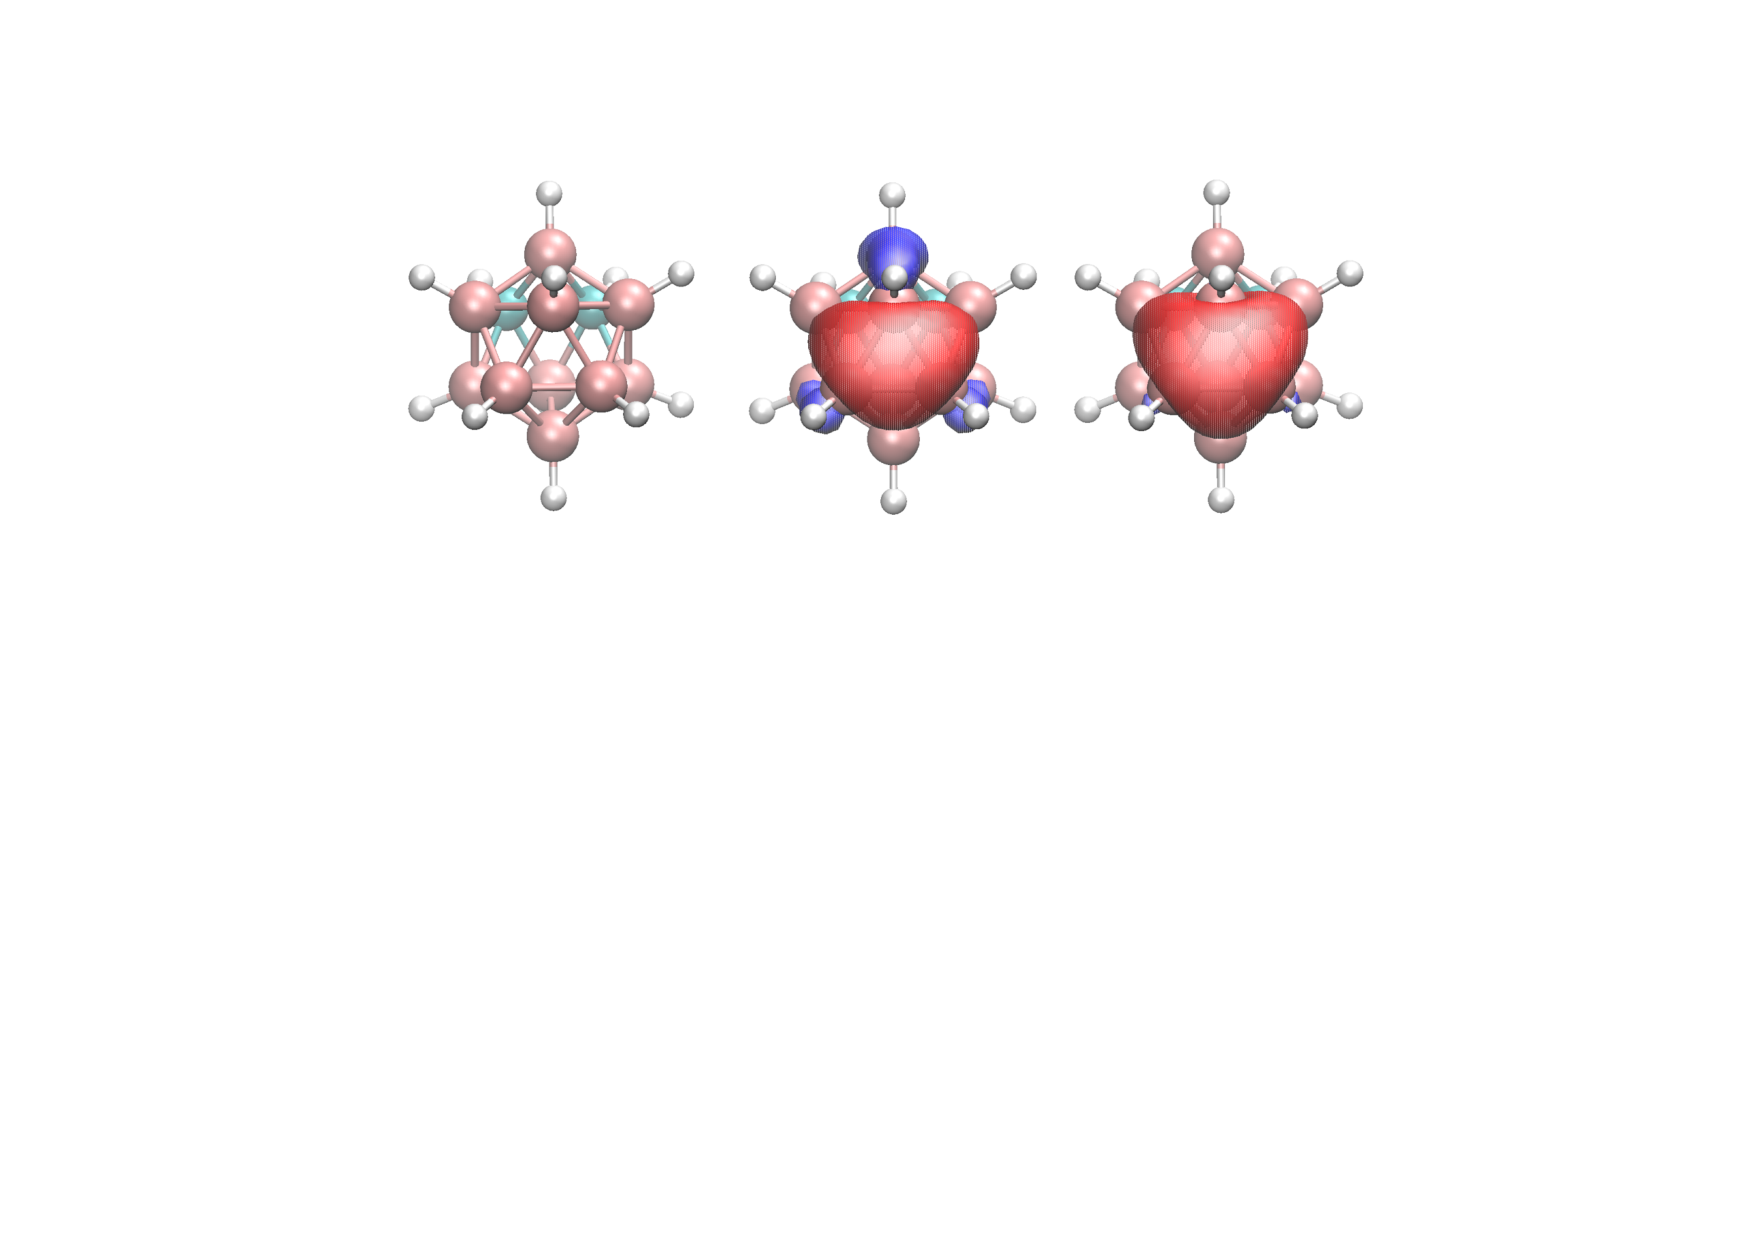
\includegraphics[scale=0.4]{carborane.pdf}
\caption{Orthogonal (bottom) and nonorthogonal (top) LMOs on the covalent bond of the two adjacent carbon atoms in a carborane molecule C$_2$B$_{10}$H$_{12}$. The isosurface value is 0.04~a.u. 
%RZK: It is not necessary to show two views of the same orbital. Replace the two right figures with the 3-center orbital, change the figure caption accordingly.
}
\label{fig:boro}
\end{figure}

Figures~\ref{fig:boro}, \ref{fig:graphene}, \ref{fig:decacyclene} and \ref{fig:pipek} compare the shapes of NLMOs and OLMOs for several representative isolated molecules and periodic systems. 
Figure~\ref{fig:boro} shows that the NLMOs and OLMOs of a carborane C$_2$B$_{10}$H$_{12}$ molecule representing a three-center two-electron B--C--B bond~\cite{melichar2018systematic} and a C--C $\sigma$-bond have similar positions of their centroids and similar overall shape. %RZK: check which oribtals we do present in the end. 
The main lobes (red region) of NLMOs are larger than those of OLMOs whereas NLMO peripheral tails are smaller. This redistribution of the probability density amplitude towards the center of NLMO is what makes NLMOs more compact than OLMOs -- the effect noted previously~\cite{liu2000nonorthogonal}. 
%Since the NLMOs have less space occupation and smaller orthogonalization tails, the main lobes should have relative larger sizes.

\begin{figure}[htbp]
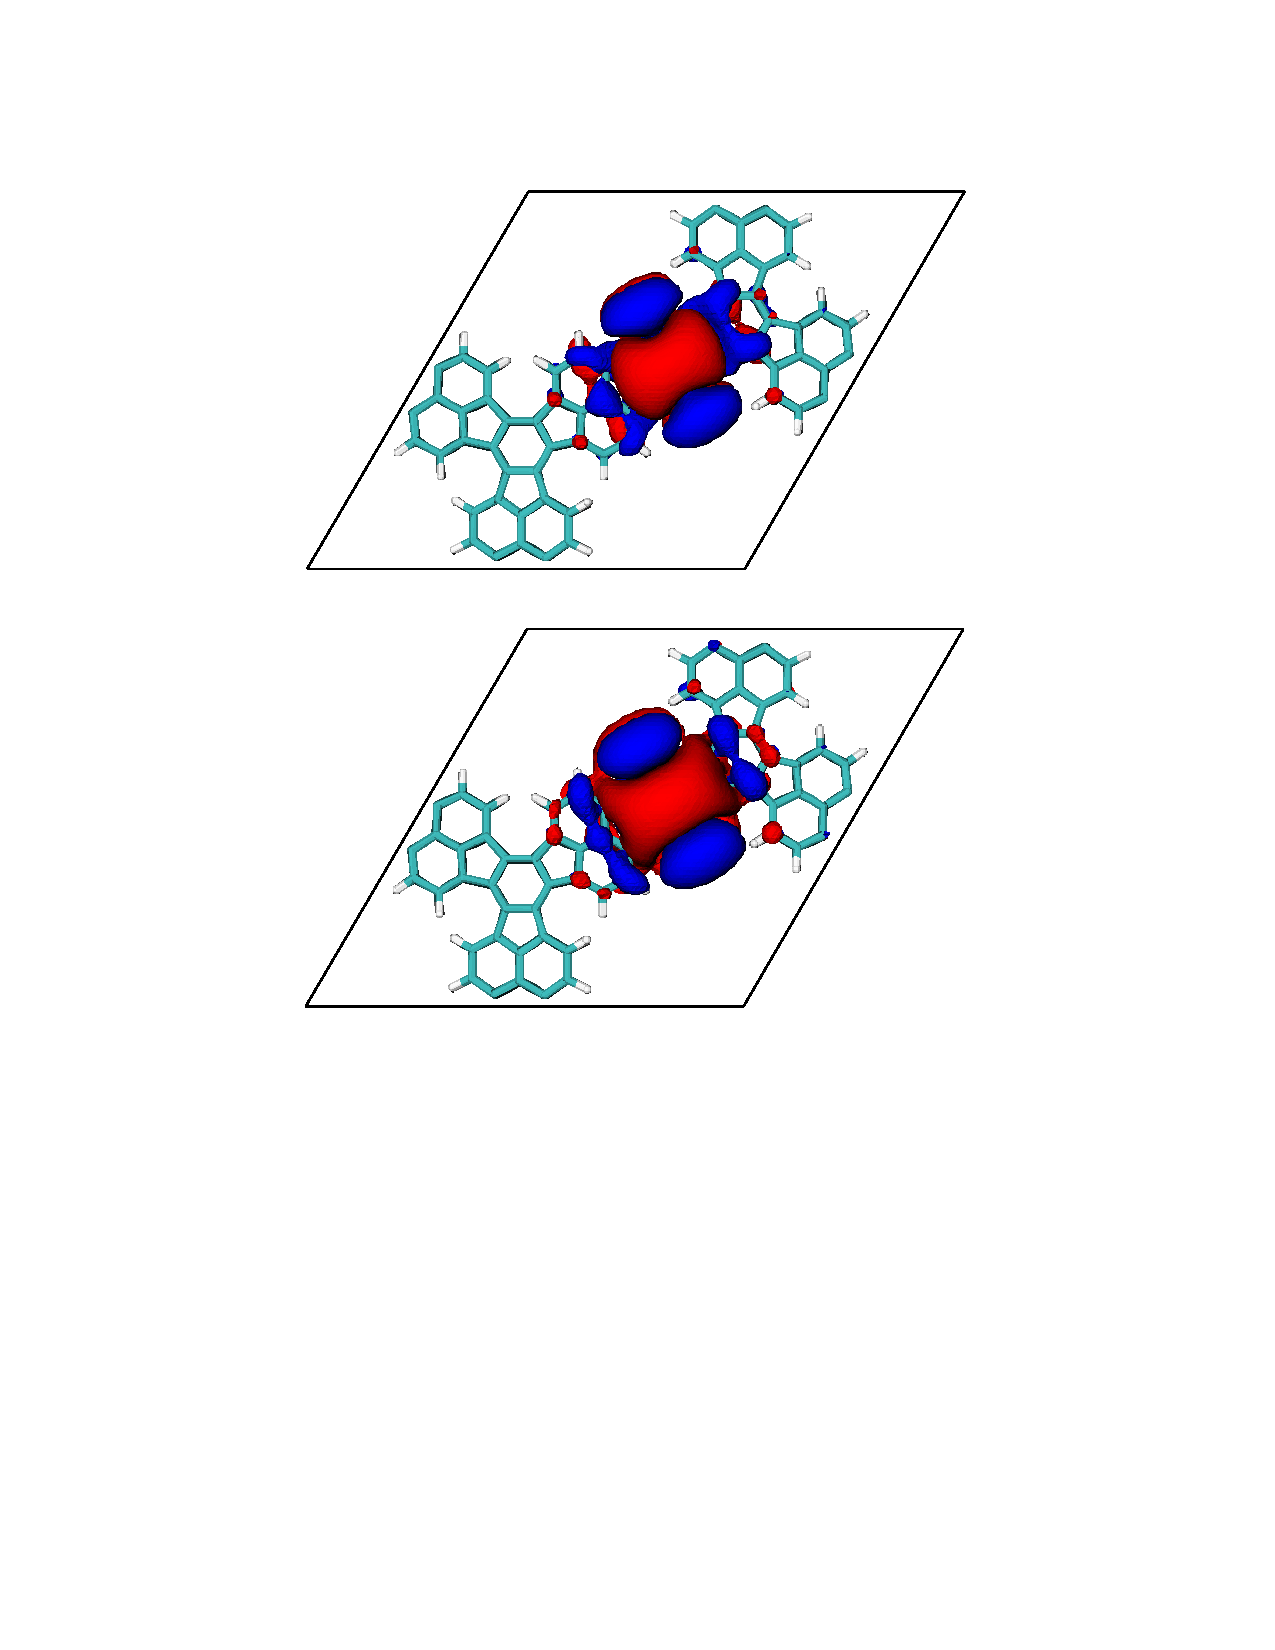
\includegraphics[scale=0.6]{figure_5.pdf} 
  \caption{NLMO (top) and OLMO (bottom) representation of a $\pi$-bond in the $\pi$-conjugated 2D polymer decacyclene C$_{72}$H$_{24}$. The isosurface value is set at a relatively low value of 0.002~a.u. to emphasize the tails of the orbitals.
%RZK: make sticks (bonds) very narrow so the tails are more clearly visible. Is it possible to make the isosurfaces more transparent so the backbone is visible?
}
\label{fig:decacyclene}
\end{figure}

The reduced tails of NLMOs are also visible in Figure~\ref{fig:decacyclene}, which shows LMO representation of a $\pi$-bond in the extended $\pi$-conjugated 2D polymer decacyclene C$_{72}$H$_{24}$. Without strict orthogonality constraints, these tails can be reduced even further by imposing higher-order (e.g. quartic) penalty on amplitudes far away from the orbital center~\cite{hoyvik2012orbital}.
%RZK https://doi.org/10.1063/1.4769866 --- Høyvik, I.-M.; Jansik, B.; Jørgensen, P. J. Chem. Phys. 2012, 137, 224114. 

\subsection{$\sigma$-$\pi$ mixing}

\begin{figure*}[hbpt]
\centering
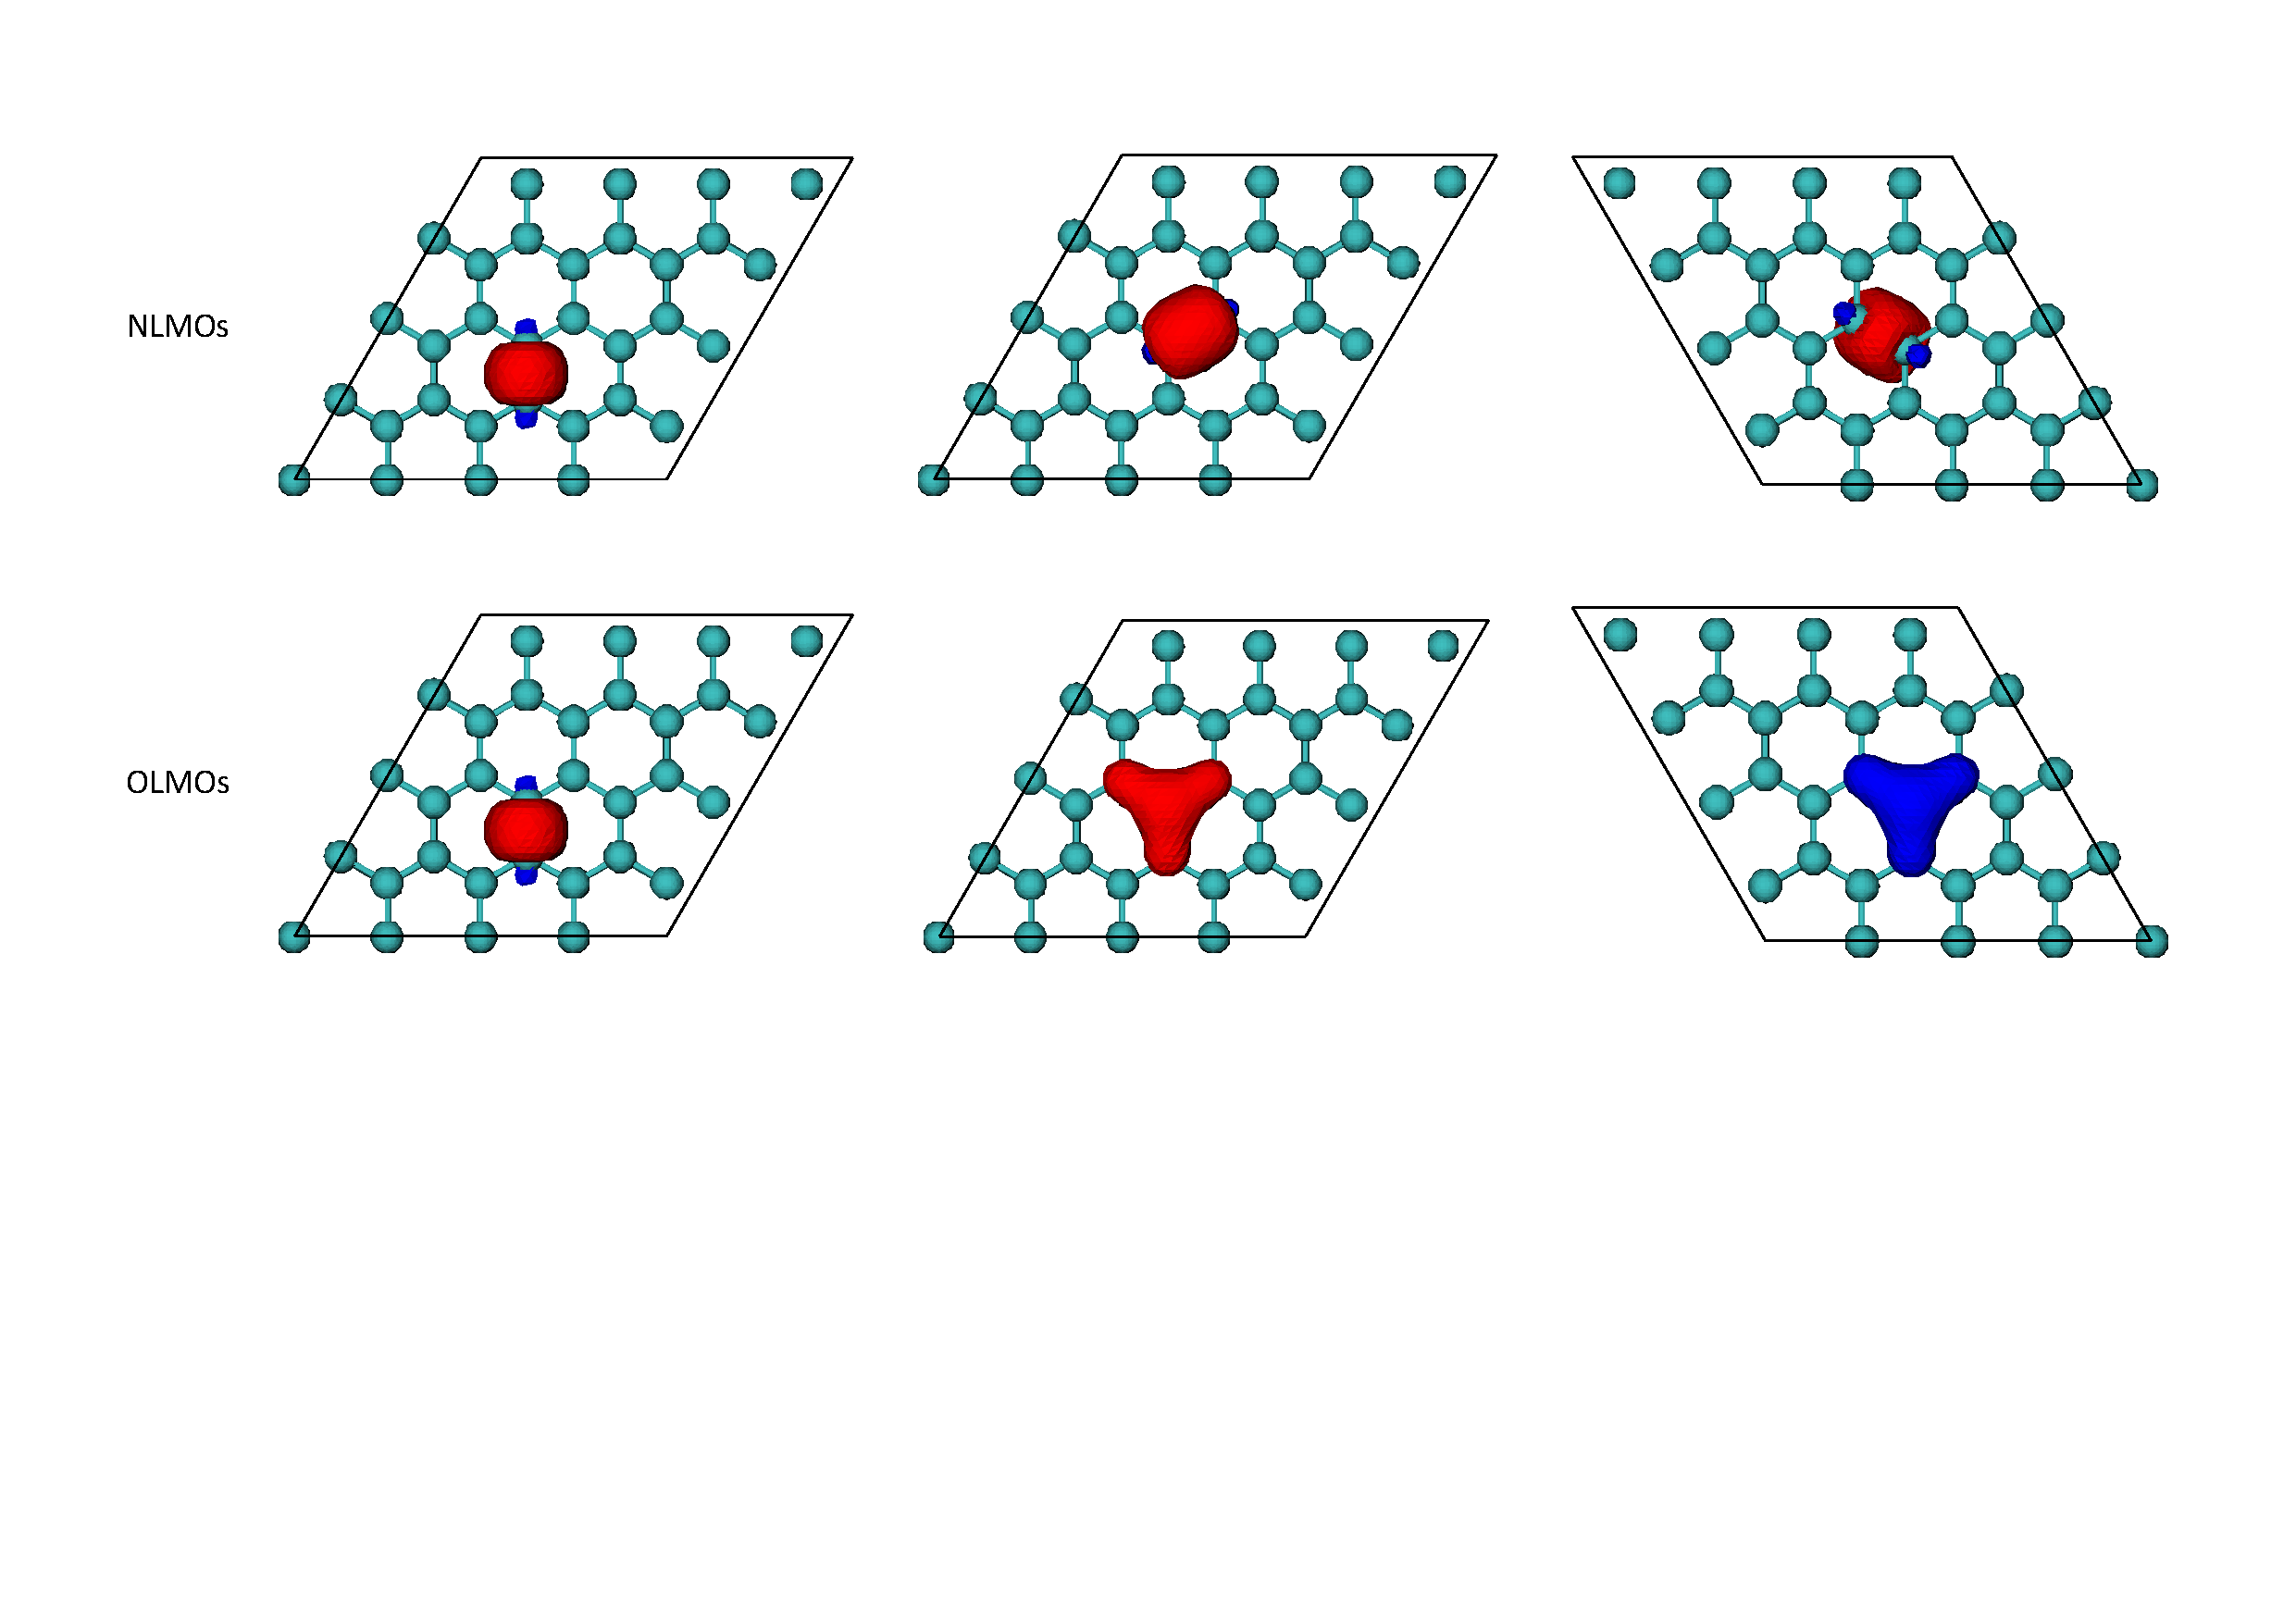
\includegraphics[scale=0.5]{figure_4.pdf}
\caption{Representative NLMOs (top) and OLMOs (bottom) of graphene. The isosurface value is 0.06~a.u.
%RZK: Remove OLMO/NLMO labels form the figure. Remove carbon spheres, leave only sticks. The rightmost column should also be removed. If we want to emphasize the sigma-pi separation/mixing side-view of all orbitals should be presented. Place the figure into a single column inside the text: figure* -> figure. 
}
\label{fig:graphene}
\end{figure*}

Figure~\ref{fig:graphene} compares typical NLMOs and OLMOs of graphene. 
The single C--C $\sigma$ bonds are well reproduced by OLMOs and NLMOs but both types of LMOs fail to represent the double bonds.  OLMOs tend to delocalize over several bonds complicating analysis of the electron pairs. Although NLMOs are more localized and extend only over two carbon atoms, they tend to take the shape of a mixture between $\sigma$ and $\pi$ bonds producing the so-called $\tau$ orbitals. To prevent the $\sigma$-$\pi$ mixing, the Berghold localization functional was replaced with the Pipek-Mezey functional. 
%RZK: we need to add Pipek-Mezey for graphene.

\begin{figure*}[htbp]
\centering
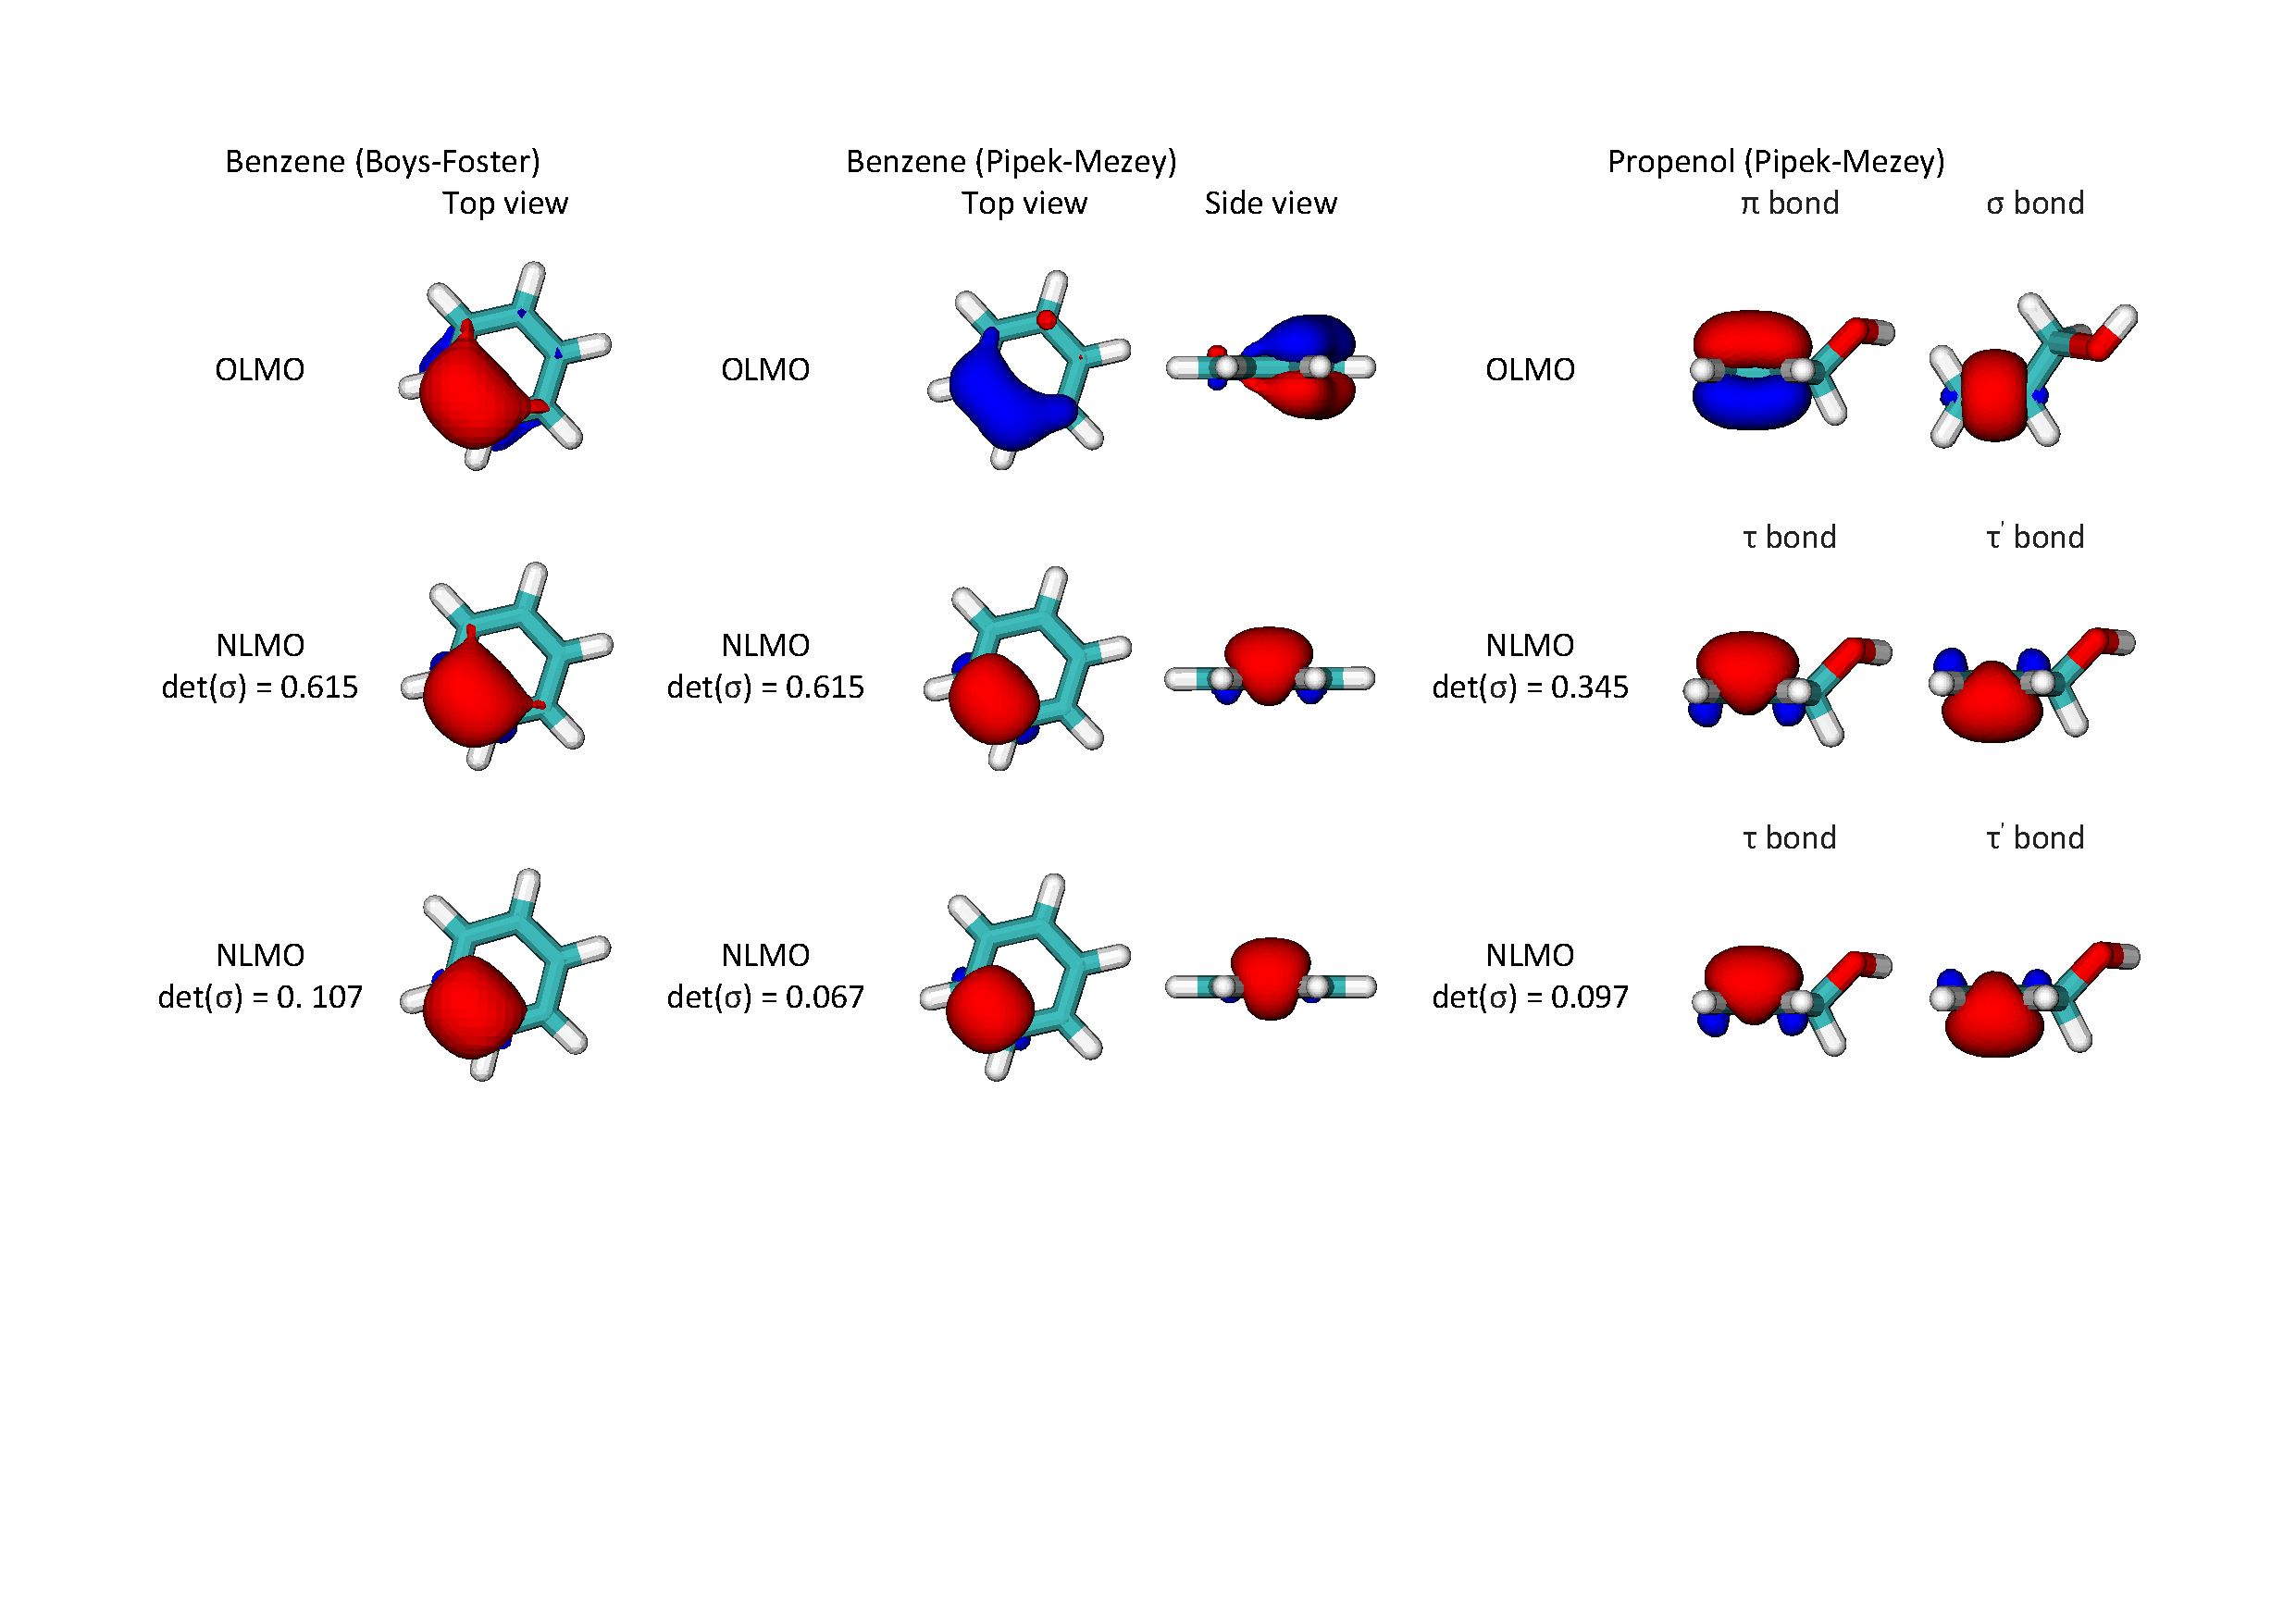
\includegraphics[scale=0.5]{figure_6.pdf}
\caption{Comparison of NLMOs and OLMOs computed with the Berghold and Pipek-Mezey localization functionals for benzene and allyl alcohol. The isosurface value is 0.05~a.u.}
%RZK: one allyl alcohol molecule is rotated differently. What is the reason for this? If there is no strong preference to dispaly it this way, make the view direction the same for all allyl alcohol molecules. Thinger sticks are required.
\label{fig:pipek}
\end{figure*}

The OLMOs and NLMOs obtained with the Pipek-Mezey and Berghold localization schemes were also compared for benzene and allyl alcohol (Figure~\ref{fig:pipek}). 
For OLMOs, the Pipek-Mezey scheme preserves the separation between the $\sigma$ and $\pi$ bonds~\cite{pipek1989fast}.
However, as the determinant of the NLMO overlap decreases the $\sigma$-$\pi$ separation of the Pipek-Mezey scheme is not maintained. 
As NLMOs become more compact a pair of $\sigma$ and $\pi$ bonds tend to mix generating a pair of $\tau$ and $\tau'$ NLMOs.  Despite the failure to preserve the $\sigma$-$\pi$ separation the Pipek-Mezey NLMOs are more localized than those obtained with the Berghold scheme.

It has been shown~\cite{RZK-pipek} that in the original Pipek-Mezey localization scheme for OLMOs $\tau$ and $\tau'$ orbitals cannot be more localized than $\sigma$ and $\pi$ orbitals
%
\begin{equation} \label{eq:OLMO-pipek}
\begin{split}
\Omega_L(\mathbf{\sigma}) + \Omega_L(\mathbf{\pi}) \leqslant \Omega_L(\mathbf{\tau}) + \Omega_L(\mathbf{\tau'})
\end{split}
\end{equation}
%
% for OLMOs preserves , the previous study has proved that the $\sigma$-$\pi$ separtion is always the stable solution compare with the mixed $\tau$ and $\tau'$ bonds for optimum population localized orbitals in Eq.~\ref{eq:pipek-tau}. 
%
Here we show using a very simple system as an example why the Pipek-Mezey localization functional can generate $\tau$ and $\tau'$ as the most localized solution 
%
\begin{equation} \label{eq:OLMO-pipek}
\begin{split}
\Omega_L(\mathbf{\sigma}) + \Omega_L(\mathbf{\pi}) \geqslant \Omega_L(\mathbf{\tau}) + \Omega_L(\mathbf{\tau'})\end{split}
\end{equation}
%
We consider a toy system of two atoms, each with (RZK: finish the description and insert relevant figures).

==== RZK: STOPPED HERE ====

The expressions of $\ket{\tau}$ and $\ket{tau'}$ of Pipek-Mezay NLMOs scheme (Eq.~\ref{eq:non-ortho-pipek}) are different from the OLMO scheme, which results in the $\pi$ and $\sigma$ separation is no longer more stable solution than the mixed case.
So that the $\sigma$ and $\pi$ seapration can not be maintained in the nonorthogonal otbitals even based on Pipek-Mezey localization functional.
%
\begin{equation} \label{eq:non-ortho-pipek}
\begin{split}
\ket{\tau} &=  \cos \theta  \ket{\sigma} + \sin \theta \ket{\pi}\\
\ket{\tau'} &= -\sin \theta' \ket{\sigma} +cos \theta' \ket{\pi}\\
\end{split}
\end{equation}



It can be seen from the Figure~\ref{fig:boro} that both OLMO and NLMO can well present the complicated bonding pattern in carborane system and the  prerequisites are no longer needed when generating NLMOs.

The study on carborane system have shown that our new approach successfully avoid using the cumbersome pre-determination and suspicious "chemical intuition" to describe the bonding pattern in the complicated and uncharted systems.

In summary, we found that NLMOs are significantly more compact and less tails than corresponding OLMOs based on our newly proposed black-box method. 
We successfully developed a new approach, which minimizes the Berghold or Pipek-Mezey localization functional and automatically self-adjusts penalty function by user specified input, to generate LMOs, especially NLMOs without the need of understanding the bonding patterns in the system or any pre-fixed/defined NLMO centers.
Our results are consistent with the previous study which the NLMOs are around $10\%$ to $30\%$ more localized than the corresponding OLMOs.
As we mentioned before, the Berghold localization functional tends to mox the $\sigma$ and $\pi$ bond during the minimization procedure, so the $\pi$ bond of NLMOs we obtained are slightly different from the traditional bonding pattern.
Further more, we surprisingly noticed that the $\sigma$-$\pi$ separation could not be preserved when generating NLMOs based on Pipek-Mezey localization scheme.
%This problem is possible to be solved if we use Pipek-Mezey~\cite{pipek1989a_fast} localization scheme.
Even though obtained NLMOs with our method have less orthogonality tails compared with conventional OLMOs, we still could observe the significantly existence of tails when using small isosurface value, which means the generated NLMOs are still not nonorthogonal enough to eliminate the tails when using second order localization functional. 
We hope this issue can be solved when applying higher order localization functional.

%RZK: isosurface value -> a.u. use words, not just "isosuface="


%Present localization paths for two systems: simple and challenging. Use $c_P$ values determined by our automatic procedure. Remember that the whole point of creating this method was to make the localization black-box.

%Can we localize virtual orbitals?

%Discuss existing issues: convergence rate, sigma-pi mixing, orthogonalization tails, sparsity of the final coefficients. Mention possible future work to resolve them.

%TODO: Visualize an xyz file with localization centers to make sure NLMOs are physical. Compute the $c_P$ coefficient correctly the equation to minimize the L2 norm of the gradient.

\section{Conclusions}
%RZZK: the algorithm is easy to implement to obtain both OLMOs and NLOMs. In the former case, it does not require to parameterize the unitary transformation.
%RZZK: it is a generalization of the proposed schemes to generate MLWFs. Important for solid state systems.
In this paper, we proposed an unconstrained and generalized black-box method to localize orbitals, especially NLMOs, that automatically determine the centers during the optimization process without any pre-understanding/defined bonding patterns in the system. 
The adjustable penalty function strength allows us to manually regulate the balance between orthogonality and locality of NLMOs.
Our calculations show that the optimization is stable and fast in our most tested systems.
With the help of the penalty function, we did not observe linear dependence issue among generated NLMOs.

Our results, which agree with previous research by Yang et al~\cite{feng2004An_efficient, cui2010efficient}, show that the NLMOs are around $7\%$ and $28\%$ more compact than the corresponding OLMOs and mostly accordance with the traditional chemical bond theory.
Also, we  can conclude that these NOLMOs can be used to present the electronic structure in the completely equivalent to the representations by the OLMOs and CMs.
Moreover, we found that the orthogonal tails are significantly reduced in the NLMOs compared with the OLMOs.
The faster tail decay for nonorthogonal orbitals is due to more degree of freedom are available without using the orthogonality constrains for nonorthogonal orbitals than orthogonal orbitals.

\section{Acknowledgments} 

The research was funded by the Natural Sciences and Engineering Research Council of Canada (NSERC) through Discovery
Grant (RGPIN-2016-0505) and by Tri-agency Institutional Programs Secretariat through New Frontiers in Research Fund (NFRFE-2018-00852). The authors are grateful to Compute Canada for computer time.

\bibliographystyle{apsrev4-1}
\bibliography{NLMOs}

\end{document}

